\documentclass{article}
% packages
\usepackage {lmodern}
\usepackage [T1]{fontenc}
\usepackage {amsmath}
\usepackage {amssymb}
\usepackage {amsfonts}
\usepackage {graphicx}
\usepackage {fullpage}
\usepackage {gensymb}
\usepackage {caption}
\usepackage {subcaption}
\usepackage {array}
\newcolumntype{L}{>{\centering\arraybackslash}m{3cm}}
%\usepackage{nopageno}
\usepackage {cite}
\usepackage {setspace}
\usepackage [version=4]{mhchem}
\usepackage {pdfpages}
\usepackage {fancyvrb}


\graphicspath {{images/}}

\begin {document} 
\title {Fourier Transform Infrared Spectroscopy on External Pertubations
Inducing Secondary Structure Changes of Hemoglobin}
\vspace{20cm} 
\author {Justin Chao - jc55395 
\\ \\ CH 456} 

\maketitle

\newpage
\section*{Project Summary}
This experiment will analyze the molecular conformational behavior of hemoglobin under
changes in temperature, and create a methodological framework for analyzing the
heat-induced behavior of similar biomacromolecules using fourier transform
infrared spectroscopy.\cite{hemo}

Bovine hemoglobin (BHb), dissolved in D$_2$O, will be assessed at incremental
temperatures using a FTIR spectrometer equipped with a MCT semi-conductor
detector. A planar silver halide fiber segment will be adapted for ATR sensing
using minute sample volumes.

The obtained spectral data will be baseline corrected and fitted using
Gaussians and adjusted parameters given by the peaks of calculated second
derivatives. By calculating second derivatives of the obtained IR-ATR spectra
along with apropriate curve fitting procedures, the contributions of individual
secondary structure elements of hemoglobin to the sum amide-I absorption feature
can be precisely allocated using Gaussian peaks.

According to literature, temperatures above 62\degree C cause $\alpha$-helix and
intermolecular $\beta$-sheet changes.\cite{hemo}

Previous experimental and computational studies have established protocols for
describing how the amide-I IR absorption is affected by the backbone structure,
including the assignment of a band at 1646 cm$^{-1}$ to $\alpha$-helix structures
a band at 1626 cm$^{-1}$ to $\beta$-sheet structures in BHb. \cite{hemo}

Therefore it is expected that at 62\degree C, peaks at 1646 cm$^{-1}$ and 1626
cm$^{-1}$ should disappear, while two new peaks should appear at 1642 cm$^{-1}$
and 1620 cm$^{-1}$, indicating the effects of temperature change on $\alpha$-helix
and $\beta$-sheet structures, leading to the formation of unordered and
intermolecular aggregates.
 

\section*{Background}
The secondary structure of proteins and other biomacromolecules are closely
related to their functions in biological systems. Any changes in the structure
may cause adverse effects to the functioning of biosystems and pathways. In this
experiment, heat-induced changes on the conformation of hemoglobin will be
studied using IR-ATR spectroscopy.\cite{Harris} This study will detail the conformational
behavior of hemoglobin under changes in temperature, and will allow for the
creation of a general methodological framework for further analysis of
heat-induced behaviors of biomacromolecules.

\section*{Goals and Objectives}
The objective of this study is to characterize the conformational changes of
hemoglobin under changes in temperature. Subsequent steps to achieve this goal
include the preparation of BHb samples, the adoption of a planar silver halide
fiber segment, the preparation of an FTIR spectrometer equipped with a
mercury-cadmium-telluride semiconductor detector cooled with liquid nitrogen,
and the analysis of the BHb samples using IR-ATR under increasing temperature
constraints. Table 1 provides a timeline of the step-wise goals towards the
completion of the study.

\begin{center}
    \captionof{table}{Timeline of goals towards study completion.}
    \begin{tabular}{l|l}
        Time    & Objective \\
        \hline
        1 week  & obtain BHb sample and prepare sample for analysis \\
        2 weeks & adopt and prepare planar silver halide fiber segment \\
        1 week  & prepare FTIR spectrometer for sample analysis \\
        2 weeks & run samples at incremental temperature constraints \\
        2 weeks & data analysis of results \\
    \end{tabular}
\end{center}

\section*{Literature Review}
Another article that supports the analytical use of IR-ATR
spectroscopy\cite{lab_man} in determining changes in the vibrational spectra of
involved species is titled "Observing non-classical crystallisation processes in
gypsum via infrared attenuated total reflectance spectroscopy" \cite{gypsum}.
In this article, the cystallization pathways of gypsum are studied via IR-ATR by
revealing detailed information on inter- and intramolecular interactions during
gypsum crystallization via changes in the vibrational spectra of the involved
reactants. This methodology is similar to how IR-ATR will be used to
characterize changes in vibrational spectra of the amide-I group in this study
on conformational changes of hemoglobin.

\section*{Methodology}
\subsection*{Experimental Procedure}
\subsubsection*{Instrumentation}
IR-ATR spectra will be obtained using a FTIR spectrometer equipped with a
mercury-cadmium-telluride (MCT) semiconductor detector cooled with liquid
nitrogen. A planar silver halide fiber segment will be adapted for ATR sensing
using minute sample volumes. Cylindrical silver halide fibers will be fabricated
by hot extrusion from a single crystal preform, which can be prepared using the
Bridgman-Stockbarger technique. After the preparation of short fiber segments by
cutting, a planar section will be constructed using a stainless-steel mold by
pressing a short cylindrical fiber section onto a planar geometry tapering into
cylindrical in- and out-coupling segments. 
The fiber will then be sealed into a flow cell equipped with a heating system
for temperature control.

In this manner, the fiber ATR sensing element is composed of cylindrical
segments at both ends, allowing for radiation in-/out-coupling with a planar active
sensing segment in the middle. Figure 2 shows an example of such an arrangement.
\begin{center}
    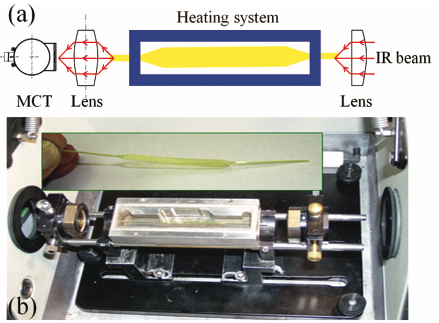
\includegraphics[scale=0.5]{segment}
    \captionof{figure}{Adapted fiber optic sensing arrangement using a
    planar-tapered silver halide fiber segment housed in a flow cell equipped
    with a heating system optically coupled to the FTIR spectrometer. (a)
    Schematic set-up and, (b) image of experimental set-up consisting of the
    planrized silver halide fiber.}
\end{center}


\subsubsection*{Sample Collection and Preparation}
Hemoglobin from bovine blood (CAS number: 9008-02-0) will be purchased from Sigma
Co., USA, and used without further purification.
Before the experiment, BHb will be dissolved in D$_2$O to a final concentration
of 0.5\% and kept for 2 days at room temperature (26$\degree$ C). D$_2$O is used
instead of H$_2$O to avoid strong H-O absorption bands within the amide-I
spectral region, while preserving the protein peak position.

Prior to sample run, each sample will be equilibrated for at least 5 min after
reaching the targeted temperature. 

\subsubsection*{Analysis}
A total of 64 scans will be averaged at a spectral resolution of 2 cm$^{-1}$ and a
frequency window of 4000 - 400 cm$^{-1}$. 
In this manner, spectra of protein samples at temperatures ranging from
26$\degree$C to 90$\degree$C in 2$\degree$C intervals will be obtained.

Given enough time, each experiment will be performed at least twice.

The given procedure of creating the flat-tapered fibers results in variations in
transducer thickness. Therefore, for each fiber an individual background
spectrum will be recorded so that comparable and self-consistent results may be
obtained, despite fiber-to-fiber variations.


\subsection*{Evaluation of Results}
Infrared spectra in the amide-I range (1600 - 1700 cm$^{-1}$) during heating
from 26$\degree$C to 90$\degree$C will be collected, baseline corrected, and
smoothed. 
It is expected that the amide-I vibration will rise with increasing temperature,
with main contributions by the C=O stretching vibration next to the NH in-plane
bending, the out-of-phase CN stretching, and the CCN deformation vibration.
These expected results may then be attributed to the peptide backbone carbonyl
stretching vibrations goverened by the interactions between the hydrogen bond and
amide units.\cite{hemo}

Due to the dependence of the backbone secondary structure on the amide-I unit,
the amide-I absorption band may be used to analyze secondary structure
conformation changes.

Second derivatives of the obtained peaks at 26, 42, 60, 84, and 86$\degree$C may
be generated in order to facilitate further curve fitting.


\section*{Modifications}
A modification that may be done to this experiment is the study on how a
decrease in temperature may effect the conformational structure changes of
hemoglobin. Rather than increasing the temperature from room temperature, the
temperature may be decreased in incremental amounts of 2$\degree$C until a final
temperature of -32$\degree$C is targeted.


\newpage
\bibliographystyle{unsrt}
\bibliography{proposal.bib}

\newpage
\section*{List of Needs}
Table 2 provides a list of materials needed for the completion of this study.

\begin{center}
\captionof{table}{List of materials needed for this study.}
    \resizebox{\textwidth}{!}{\begin{tabular}{l|c|c|c|c|c}
    Name & CAS Number & Vendor Name & Cost of Item & Amount & Quantity Needed \\
    \hline
    Vector 22 FTIR Spectrometer & - & Bruker Optics & - & 1 & 1 \\
    MCT Semiconductor Detector & - & Bruker Optics & - & 1 & 1 \\
    Heating/Magnetic Stir Plate & - & Benchmark Scientific & \$352.50 & 1 & 1 \\
    Micro Stir Bar & - & Cole-Parmer & \$5.62 & 1 & 2 \\
    Pyrex\textsuperscript{\textregistered} test tubes & - & Sigma Co. & \$47.60 & 72 & 5 \\
    Brand\textsuperscript{\textregistered} test tube rack & - & Sigma Co. & \$77.00 & 1 & 1 \\
    Nichiryo pipette tips (200 $\mu L$) & - & Sigma Co. & \$14.00 & 1000 & 64 \\
    Nichipet Eco pipette & - & Sigma Co. & \$428.90 & 1 & 1 \\
    Pyrex\textsuperscript{\textregistered} Griffin beaker (50 mL) & - & Sigma Co. & \$59.90 & 12 & 5 \\
    Digital Thermometer (-50.0 - 199.9$\degree$C) & - & Sigma Co. & \$103.5 & 1 & 1 \\
    Silver Bromide (99\%) & 7785-23-1 & Sigma Co. & \$43.50 & 5 grams & 5 grams \\
    Deuterium Oxide (99.9 atom\% D) & 7789-20-0 & Sigma Co. & \$23.00 & 10 grams & 4 grams \\
    Liquid Nitrogen & 7727-37-9 & Airgas & \$10 & 2 L & 1 L \\
    Bovine Blood & 9008-02-0 & Sigma Co. & \$116.50 & 5 grams & 4 grams \\
    \end{tabular}}
\end{center}

\newpage
\section*{Supporting Articles}
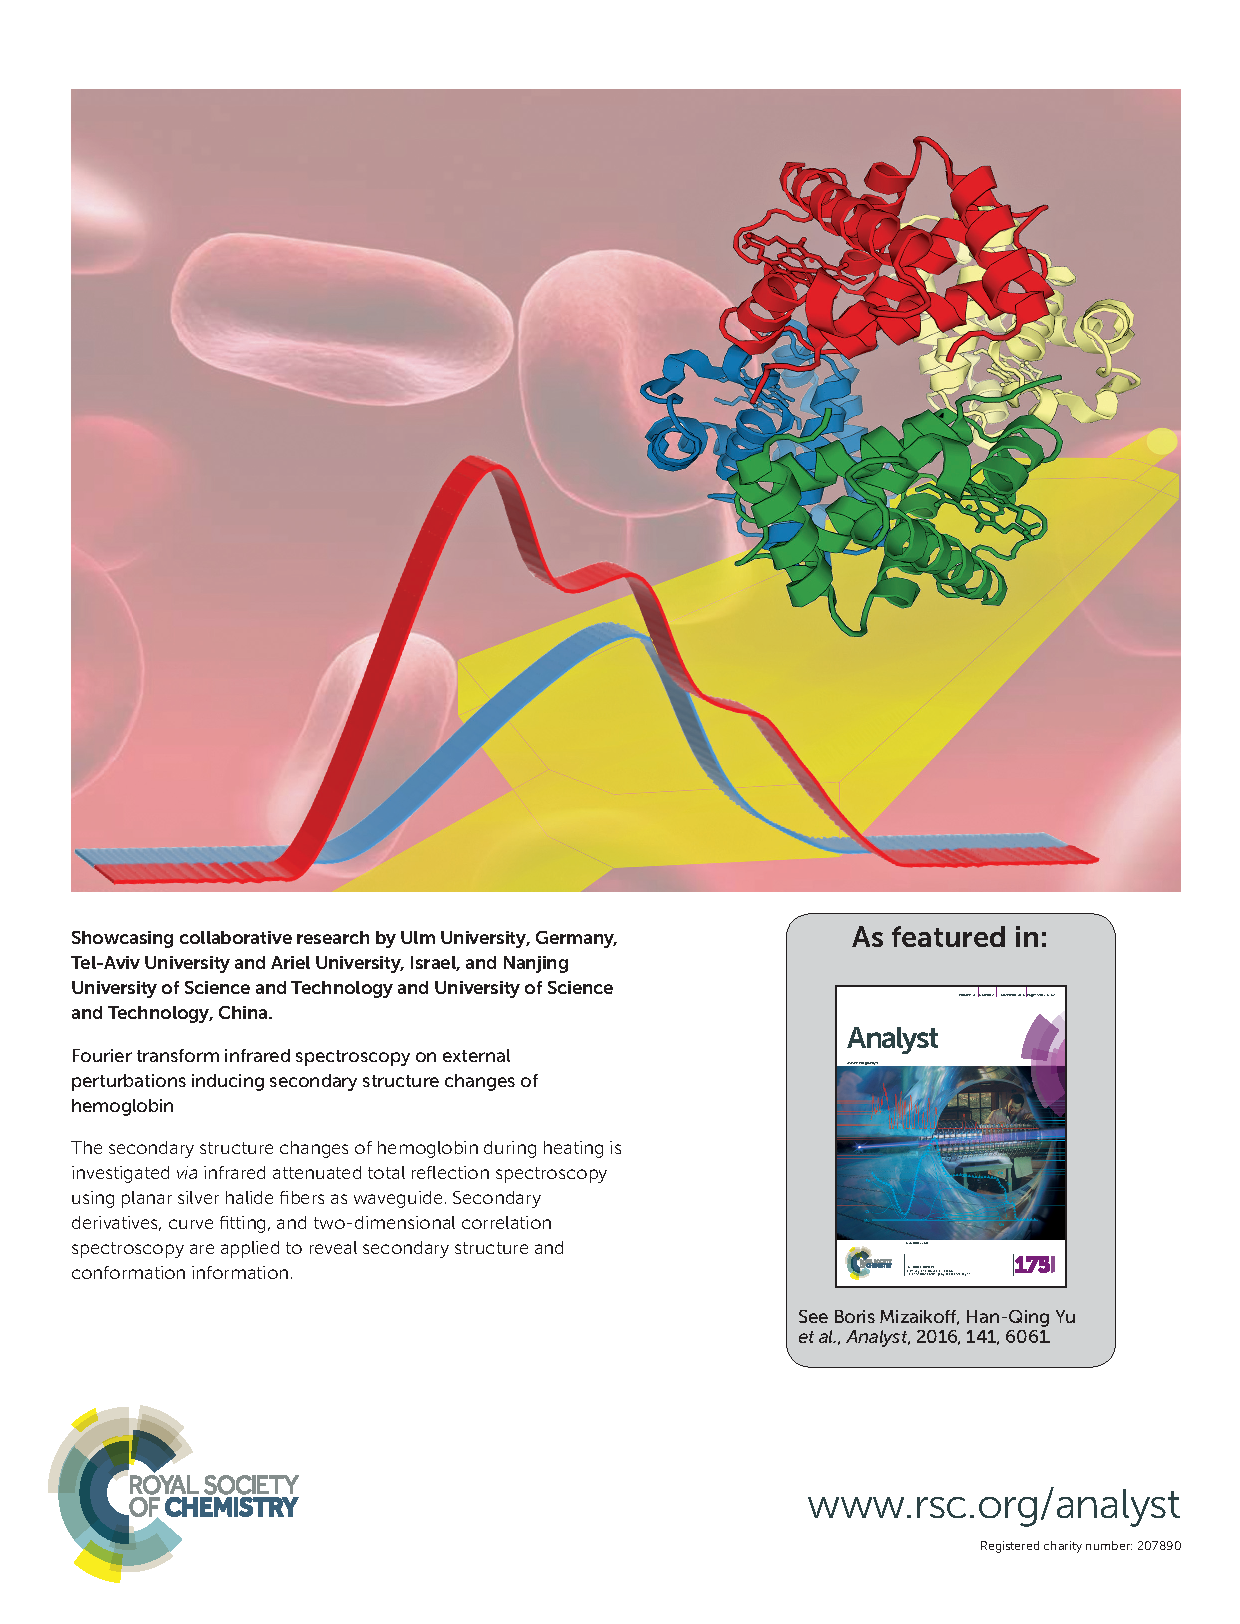
\includepdf[pages=-, pagecommand={}]{hemoglobin_FTIR.pdf}
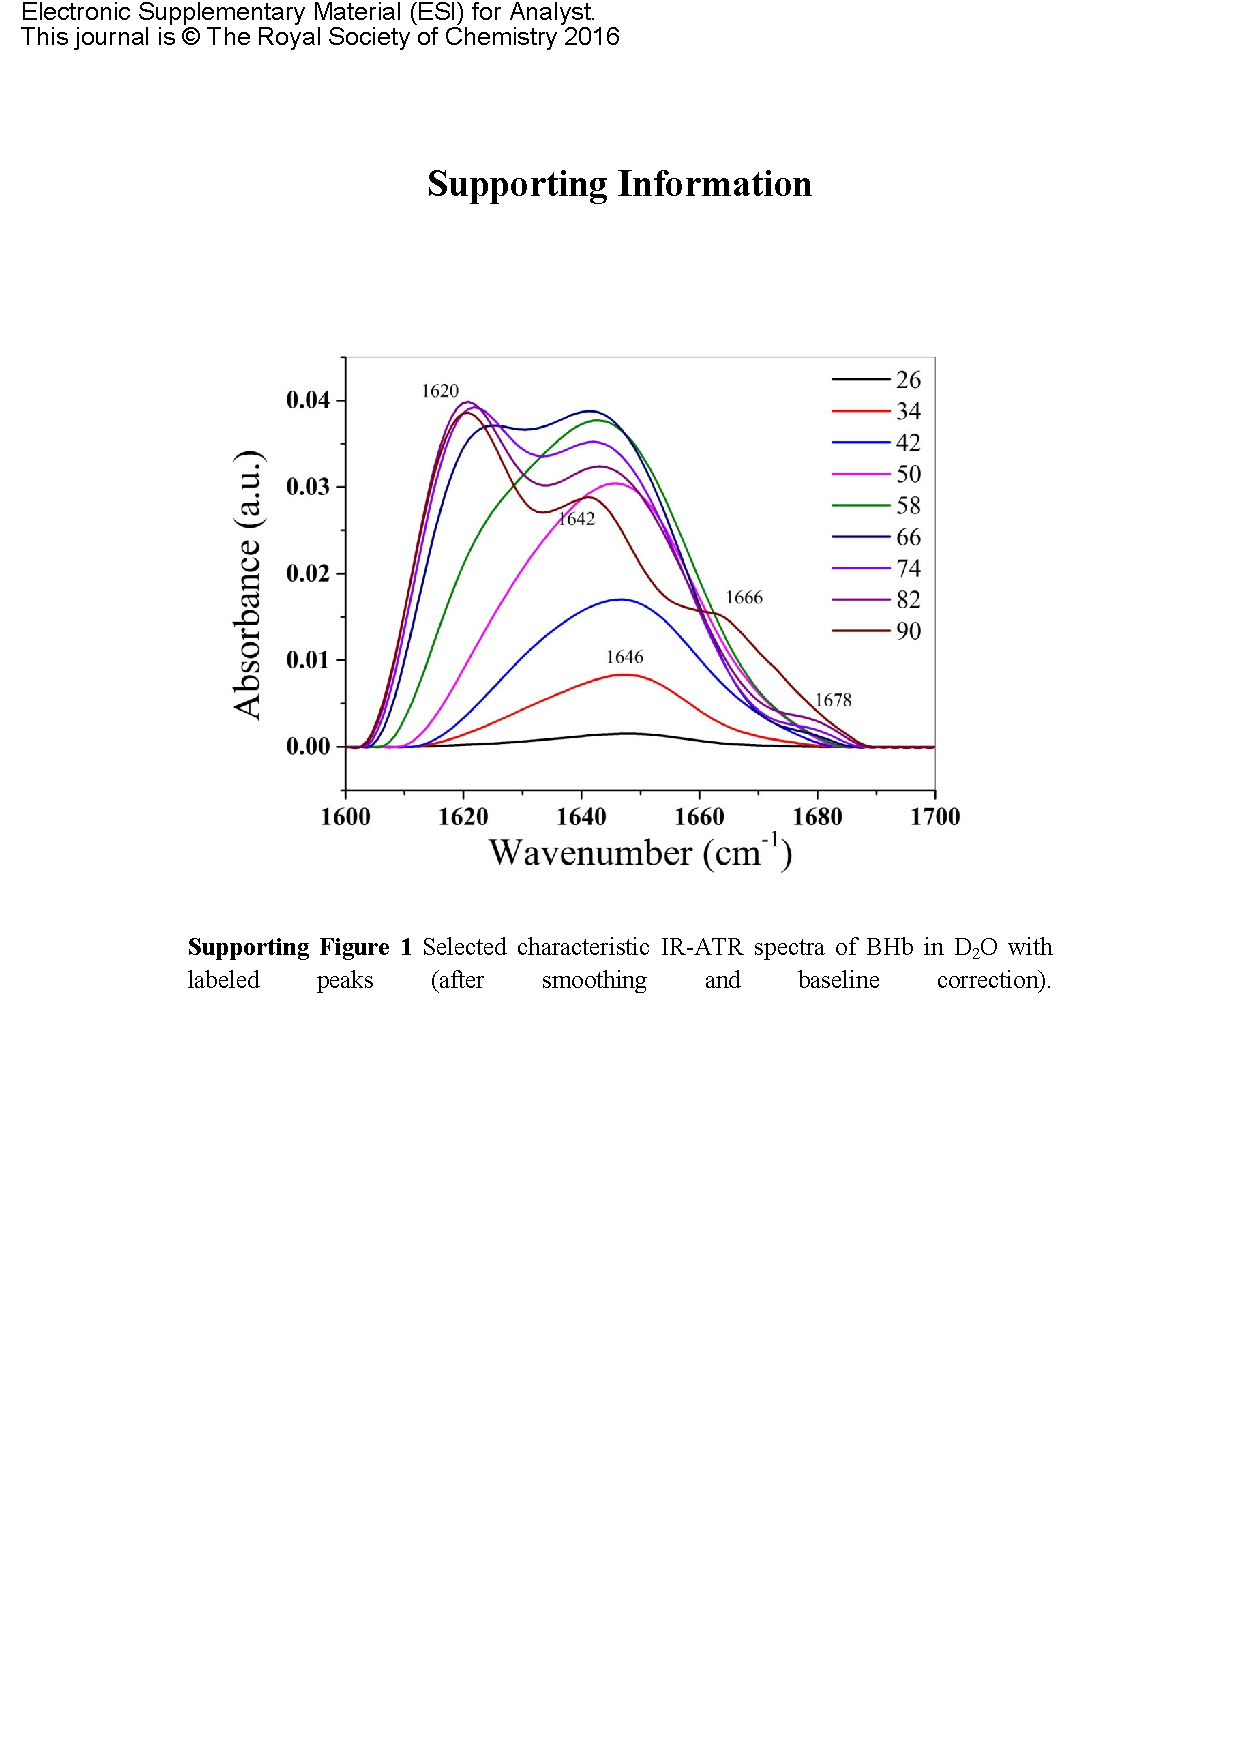
\includepdf[pages=-, pagecommand={}]{esi.pdf}
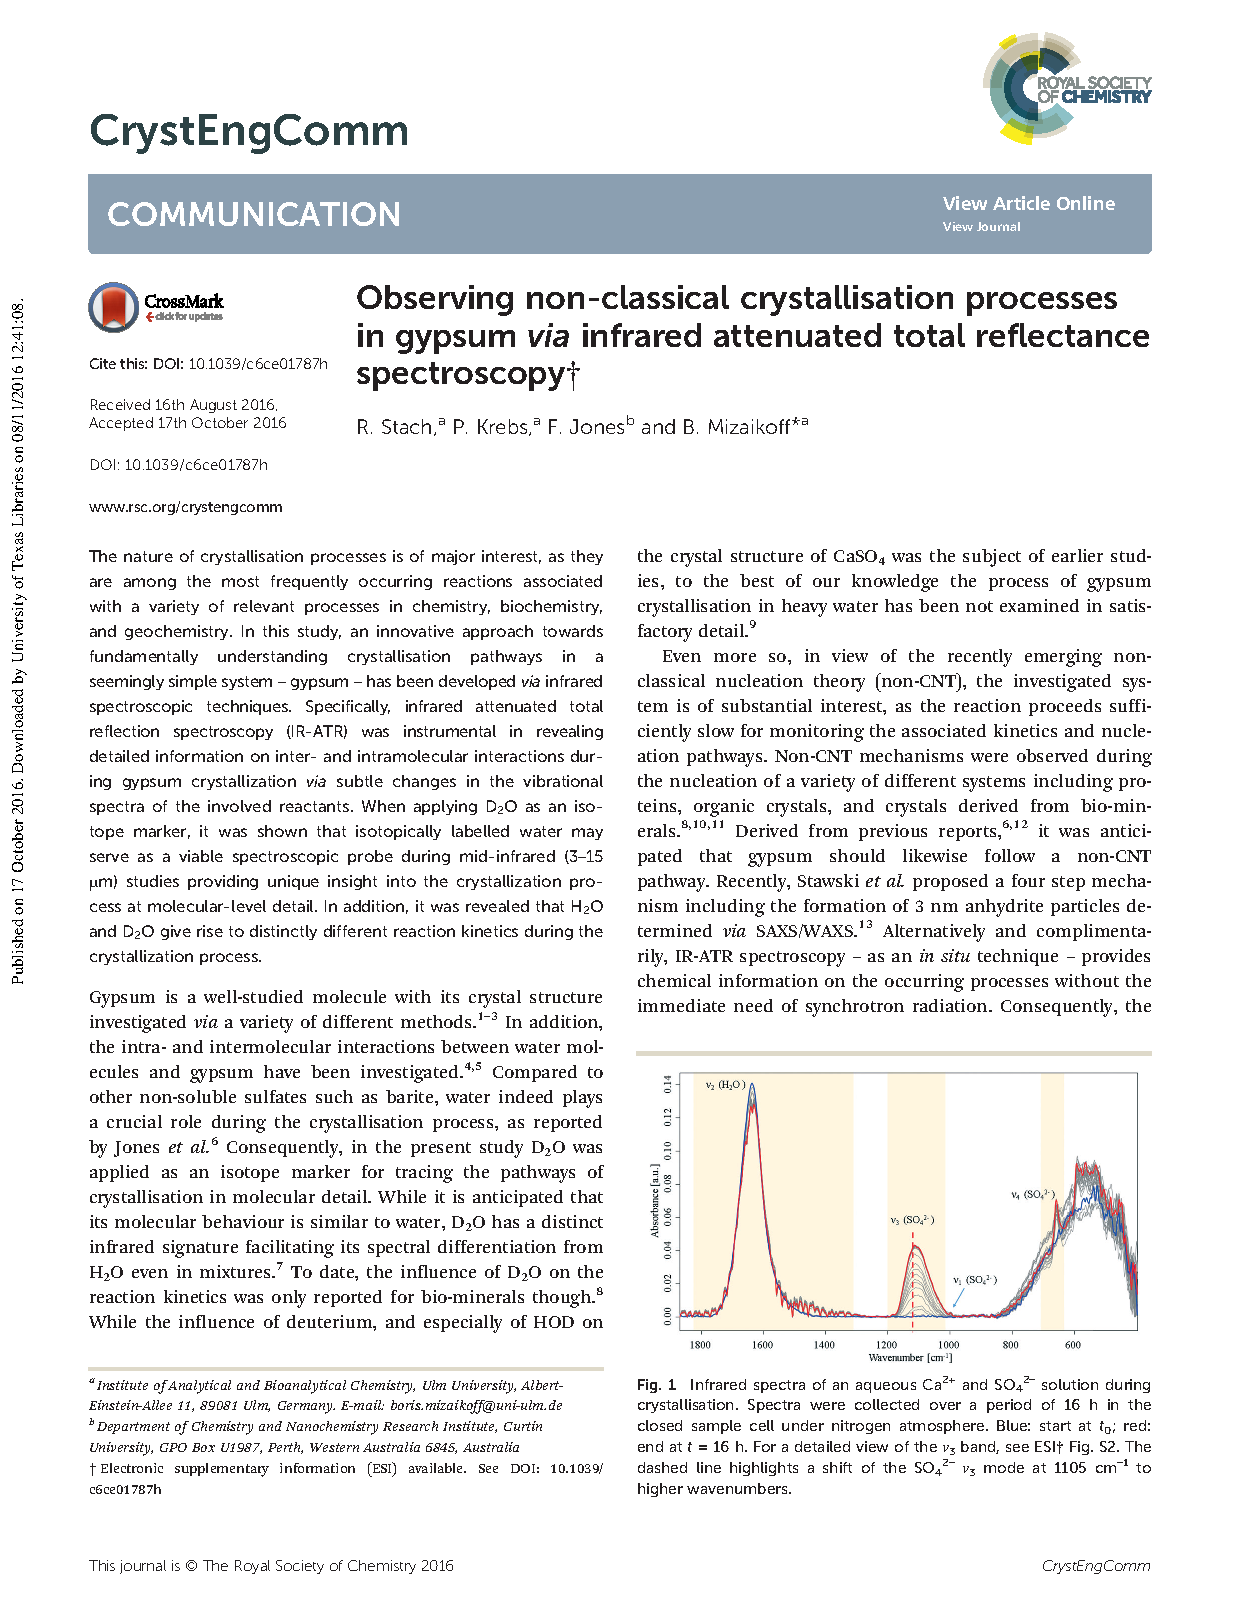
\includepdf[pages=-, pagecommand={}]{gypsum.pdf}
\end {document}
